\section{Ovládání 230V periferií}
\label{sec:perif-230v}
Jak vyplývá z~požadavků zařízení a přehledu používané akvaristické techniky, pro automatizovaný provoz akvária je nutné umožnit řídicí jednotce ovládat několik okruhů se síťovým napětím a spínat tak zvlášť zakoupené hotové spotřebiče pracující s~tímto napětím. Jedná se typicky o~ohřev vody, filtraci, popř. některé druhy osvětlení. 

\begin{figure}[h!]
    \centering
    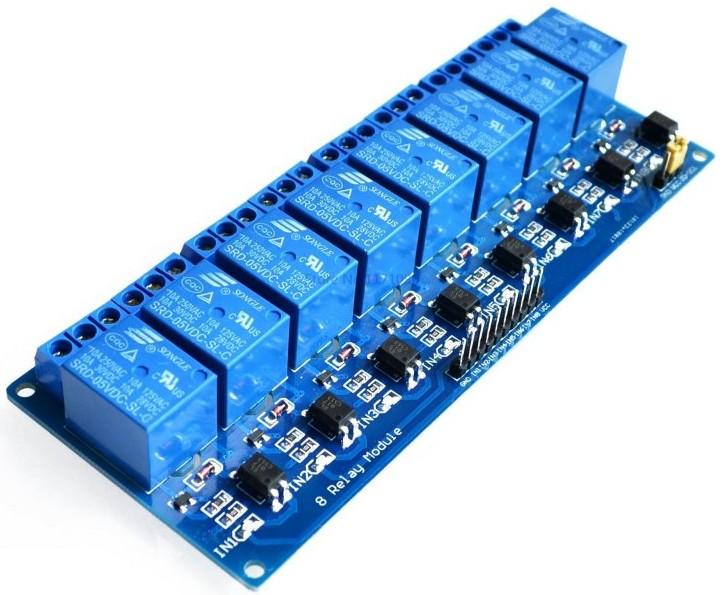
\includegraphics[width=0.6\textwidth]{obrazky/230/rele.jpg}
    \caption{TODO vyměnit: Relé modul, ilustrační foto. Převzato z~\cite{eshop-laskakit-rele}.}
    \label{fig:obrazky-230-rele-jpg}
\end{figure}


Aby uživatel mohl spínaná zařízení bezpěčně připojit bez nutnosti odborné způsobilosti, nachází se na hlavním šasi zařízení čtyři standartní zásuvky (typ E) s~jednofázovým napětím \qty{230}{V}. Fázové vodiče jsou uvnitř zařízení přerušeny spínacími relé. Je použit předpřipravený modul disponující osmi relé~\cite{eshop-laskakit-rele}, čtyři z nich tedy zůstanou nevyužité a slouží jako rezerva pro případ poškození některého z~používaných relé nebo při potřebě budoucího rozšíření o~další zásuvky. 

Z~důvodu nedostatku pinů na mikrokontroléru řídicí jednotky (ESP32) je k~relé modulu připojen ještě jeden externí modul a to expandér GPIO pinů komunikující přes sběrnici \acs{i2c}~\cite{eshop-laskakit-expander}. Z~pohledu mikrokontroléru jsou tak všechny zásuvky ovládány pomocí dvou GPIO pinů (SDA, SCL), které je navíc možné dále využít pro připojení jiných periferií jako např. OLED displaje pro zobrazení stavu zařízení.

Relé na použitém modulu potřebuje pro spolehlivé sepnutí napětí alespoň \qty{5}{V}, logické signály řídicí jednotky ale pracují s napětím pouze \qty{3.3}{V}. Ze schématu na obr.~\ref{fig:relay-board-simp-schema} je vidět, že použitý relé modul je spínán signálem logické nuly, tímto způsobem je problém s rozdílnou úrovní napájení elegantně vyřešen. 

\begin{figure}[h!]
    \centering
    % trim=left bottom right top
    \includegraphics
    [
        width=\textwidth, 
        page=3, 
        trim=2.5cm 14.5cm 18cm 1.5cm, 
        clip
    ]{obrazky/exportovane/ukazky-do-textu.pdf}
    \caption{Schéma jednoho kanálu relé modulu. Vytvořeno v~KiCad 7.0.}
    \label{fig:relay-board-simp-schema}
\end{figure}

Do budoucna by bylo možným zlepšením a rozšířením této práce zahrnutí obou zmíněných modulů přímo na DPS řídicí jednotky. 